\section{На опыте}

\begin{frame}{Тестирование производительности робототехнических фреймворков}
	\begin{itemize}
		\item Постановка задачи
		\item Выбор инструментов
		\item Реализация
		\item Проблемы
		\item Продолжение реализации
		\item Результаты
	\end{itemize}
	\centering
	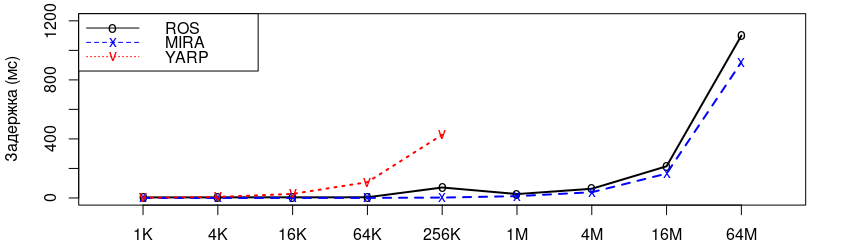
\includegraphics[height=3cm]{img/robots.png}
\end{frame}

\begin{frame}[fragile]{Программный монитор для КМПО}
			\begin{itemize}
				\item Предыстория
				\item Постановка задачи
				\item Проблемы и решения
				\item WIP
			\end{itemize}
		\tiny
	\begin{lstlisting}
#define STORE_STATE()  \
__asm__ __volatile__("mov %0, rsp;\n\t" : "=m"(VenusTestLib::MacrosOnly::directInstance._rsp));          \
__asm__ __volatile__("mov %0, rbp;\n\t" : "=m"(VenusTestLib::MacrosOnly::directInstance._rbp));          \
__asm__ __volatile__("mov %0, rbx;\n\t" : "=m"(VenusTestLib::MacrosOnly::directInstance._rbx));          \
__asm__ __volatile__("mov %0, r12;\n\t" : "=m"(VenusTestLib::MacrosOnly::directInstance._r12));          \
__asm__ __volatile__("mov %0, r13;\n\t" : "=m"(VenusTestLib::MacrosOnly::directInstance._r13));          \
__asm__ __volatile__("mov %0, r14;\n\t" : "=m"(VenusTestLib::MacrosOnly::directInstance._r14));          \
__asm__ __volatile__("mov %0, r15;\n\t" : "=m"(VenusTestLib::MacrosOnly::directInstance._r15));          \
__asm__ __volatile__("lea %0, [rip - 0x7];\n\t" : "=r"(VenusTestLib::MacrosOnly::directInstance._rip));  \
__asm__ __volatile__("mov r12, %0;\n\t" : : "m"(VenusTestLib::MacrosOnly::directInstance._r12));         \
__asm__ __volatile__("mov r13, %0;\n\t" : : "m"(VenusTestLib::MacrosOnly::directInstance._r13));         \
__asm__ __volatile__("mov r14, %0;\n\t" : : "m"(VenusTestLib::MacrosOnly::directInstance._r14));         \
__asm__ __volatile__("mov r15, %0;\n\t" : : "m"(VenusTestLib::MacrosOnly::directInstance._r15));         \
__asm__ __volatile__("mov rbx, %0;\n\t" : : "m"(VenusTestLib::MacrosOnly::directInstance._rbx));         \
__asm__ __volatile__("mov rsp, %0;\n\t" : : "m"(VenusTestLib::MacrosOnly::directInstance._rsp));         \
__asm__ __volatile__("mov rbp, %0;\n\t" : : "m"(VenusTestLib::MacrosOnly::directInstance._rbp));         \
#define RESTORE_STATE()                                                                         \
__asm__ __volatile__("jmp %0;\n\t" : : "m"(VenusTestLib::MacrosOnly::directInstance._rip)); \
\end{lstlisting}
\end{frame}

\section{Материалы}
\begin{frame}{Книги и доклады}
	\begin{itemize}
		\item Главное действующее лицо: Brendan Gregg (Netflix) с  \href{http://www.brendangregg.com/index.html}{\beamerbutton{сайтом и блогом}} и книгой Systems Performance Enterprise and the Cloud (2014)
		\setbeamercolor{button}{fg=white,bg=red}
		\item Chandler Carruth (Google) \href{https://youtu.be/nXaxk27zwlk}{\beamergotobutton{Tuning C++: Benchmarks, and CPUs, and Compilers! Oh My!}}
		\item Александр Алексеев (Postgres Professional)  \href{https://youtu.be/0NU07havVD0}{\beamergotobutton{Профилирование кода на C/C++ в *nix-системах}}
		\item Кирилл Борисов (Яндекс)  \href{https://youtu.be/pa_kAkXuOyA}{\beamergotobutton{Flame graph новый взгляд на привычное профилирование}}
	\end{itemize}
\end{frame}

\begin{frame}{Заключение}
	\begin{columns}
		\begin{column}{.3\textwidth}
			Тестирование производительности ресурсозатратно, дорого, требует много знаний и сил... но порой и очень интересно
		\end{column}
		\begin{column}{.7\textwidth}
		\begin{flushright}
				\includegraphics[height=\textheight]{img/meme.png}
		\end{flushright}
		\end{column}
	\end{columns}

\end{frame}